\documentclass[a4paper,11pt]{article}
\usepackage{headerlatex}

\title{Description du projet de Réalité Virtuelle}
\date{\today}
\author{Maxime Heme ()  \and Nicolas Pellissier (1592908)}
\begin{document}
\maketitle
\section*{Introduction}
Le projet que l'on souhaite realiser a pour objectif de recreer une ville entiere, principalement compose de buildings, dans laquelle on pourrait s'imerger et naviguer aussi bien dans les rues qu'avec une vue aerienne.
De plus, le choix d'un mode Jour/Nuit sera  utilise, c'est-a-dire que l'utilisateur pourra choisir de naviguer dans la ville de jour

\section {Affichage d'objets 3D}

Cette partie présente l'organisation de l'affichage 3D de notre application.
\subsection{Objets affichés}
Les objects affiches seraient donc de 2 natures differentes. Les objets visibles lors d'une navigation aerienne seraient des buildings de differentes tailles et differentes formes, formant un espace homogene qui constituerait une ville.
Lors de la navigation a l'interieur de la ville, nous verrions donc les details de ces buildings, ainsi que les rues qui constituent le sol de la ville, et quelques details tels que des lampadaires et quelques voitures. 

\subsection{Objets créés}
Les objets presents au lancement du programme seraient les buildings, avec un nombre suffisants de ceux-ci pour donner l'impression d'une ville. 
Lors de la navigation aerienne, d'autres buildings seront regeneres afin de ne pas atteindre les limites de la ville rapidement, mais la ville possedera des limites, qui seront mises en evidence par l'arrivee sur la mer. En effet, la ville pourra donner l'impression d'etre situee sur une ile.
Les objets tels que rues, lampadaires ou voitures seront crees lors du passage a la navigation interieure a la ville.

\subsection{Géométrie des objets}
La geometrie des objets sera simple de base, et pourra etre amelioree si le temps le permet. Pour creer les buildings, il nous faudra creer une base simple a partir de formes geometriques simples, auxquelles on donnera du volume, et que l'on "empilera" pour faire les differents etages.

\subsubsection{attributs}
Les attributs (couleurs, lumieres, textures...) seront definis de facon a ce que le rendu de la ville soit ressemblant a une ville actuelle. 
\begin{itemize}
\item couleurs
\item lumières
\item textures
\item environnement
\end{itemize}

\subsubsection{Utilisation listes d'affichages}

Les listes d'affichage seront utilisees de la maniere suivante : 
    Une liste d'affichage comprendra le volume de base d'un building, et sera ainsi utilisee pour dupliquer de facon verticale ce volume, afin de constituer les differents etages de ce building.  Nous pourrons ainsi generer des buildings de meme forme, mais de tailles differentes. 
\section{Navigation}

\subsection{Point de vue du monde}
Le point de vue du monde pourra se faire de deux manières différentes.

\begin{itemize}
\item une vue derrière le vaisseau qui permettra de diriger le vaisseau plus facilement à travers la ville
\item une vue avec le nez du vaisseau en premier plan
\end{itemize}

Le mode de vue sera défini par le choix d'un paramètre au lancement de l'application.

\subsection{Déplacement dans le monde}
    
Les déplacements se feront à l'intérieur d'un vaisseau. L'utilisateur se déplacera en volant à travers le monde, il sera complètement libre de se déplacer dans le monde à vol d'oiseau. 
Le vaisseau ne pourra pas traversé les éléments fixes du monde comme tous les immeubles le sol et l'eau représeantant les limites du monde qui entoure le monde.
 
\subsection{Degré de réalisme envisagée}

l'environnement à l'intérieur de la ville sera quasiment vide. Seul quelques voitures seront garés à certains endroits et des lampadaires seront disposer dans les rues. Il n'y aura pas d'autre vaisseau en mouvement dans la ville. La gravité ne sera pas utilisé lorsque le vaisseau est à l'arret il effectue un vol stationnaire, il ne tombera pas. Les fenêtres des immeubles seront réfléchissante.
 
\section{Interaction avec l'utilisateur}
\subsection{Utilisation du wand et des boutons}
\subsubsection{Les boutons du wand}
le vaisseau se déplace a une vitesse minimal constante initialement. Si la gachette («bouton1») est appuyé la vitesse de déplacement du vaisseau augmente jusqu'à une limite maximale. Si on relache la gachette la vitesse diminue
jusqu'à redevenir minimal.

Le bouton gauche («bouton 2») permettra d'arreter complètement le vaisseau et de lui faire affectuer un vol stationnaire.

 
\subsubsection{orientation du wand}
\begin{itemize}
\item incliner vers l'avant fait descendre le vaisseau;
\item incliner vers l'arriere fait monter le vaisseau;
\item incliner vers la gauche fait tourner le vaisseau vers la gauche;
\item incliner vers la droite fait tourner le vaisseau vers la droite;
\end{itemize}

Il sera possible de tourner à gauche et de monter en inclinant le wand vers la gauche et vers l'arrière en meme temps.

 
\section{Son}
Pour rajouter au realisme de la ville et pour accentuer l'effet de realite virtuelle, une modelisation sonore sera ajoutee. 
Elle comprendra des bruitages dues aux collisions, un bruit de fond constant lors des deplacements qui pourra donner l'impression d'etre dans un vaisseau lors de la navigation (possiblement helicoptere)
Ce bruit de fond pourra etre accentue pendant les periodes d'acceleration et diminue pendant  les periodes de decelaration.
Lors de la navigation interieure a la ville, un environnement sonore sera present sous forme de bruit de fond, simulant le bruit sonore des grandes villes (bruit de voitures, klaxons, animations diverses...)
Une musique d'ambiance pourrait etre ajoutee lors de la navigation aerienne.
 
\section{Implantation informatique}
Nous comptons utiliser Blender pour modéliser nos forme de bases permettant de génerer les immeubles puis la ville. Pour cela nous ne sommes pas encore absolument certains mais nous pensons exporter les modèle dans un format Wavefront (.obj) que OpenSceneGraph peut ouvrir. Ce choix de format n'est pas encore définitif puisque ce n'est pas le plus optimal pour des formes un peu plus complexe le chargement est assez long.

 
\section{Idées supplémentaires}
Ici nous allons décrire les idées que nous aimerions àjouter à notre environnement de réalité virtuelle si le temps nous le permet

\subsection{Alternance entre jour et nuit}
Le bouton droit («bouton 3») permettra de passer du jour à la nuit. Ainsi on pourra changer complètement l'impact de la ville. Les fenetres des buildings seront éclairés aléatoirement pour donner un effet plus vivant à la ville. Les lampadaires feront remonter la lumière comme un halo de loin.
\begin{itemize}
\item Ciel uniformément bleu le jour / Étoilé la nuit
\item environnement vide nous sommes les seules, pas de piétons dans la ville (peut etre ajouter une ou deux voitures).
\end{itemize}
 
\section*{Conclusion}

Pour illustrer ce a quoi nous souhaiterions que notre projet ressemble, voici deux courtes videos à partir desquelles nous avons tirées nos principales idées pour ce projet.
\begin{figure}[h!]
  \centering

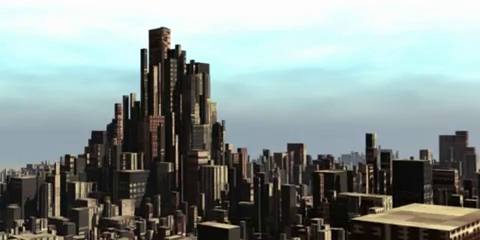
\includegraphics[width=0.7\textwidth]{images/shot0003.png}
  \caption{la ville de jour}
  \label{fig:villes1}
\end{figure}
\begin{figure}[h!]
  \centering

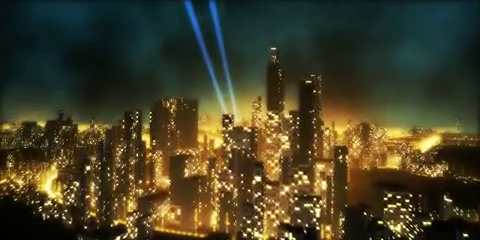
\includegraphics[width=0.7\textwidth]{images/shot0005.png}
  \caption{la ville de nuit}
  \label{fig:villes2}
\end{figure}
\begin{figure}[h!]
  \centering

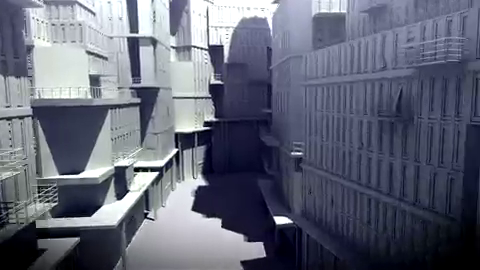
\includegraphics[width=0.7\textwidth]{images/shot0006.png}
  \caption{la ville de l'intérieur}
  \label{fig:villes3}
\end{figure}
%http://www.youtube.com/watch?v=HROU3gLcgfg&feature=related

%http://www.youtube.com/watch?v=N0LDnz-gq_o&NR=1 


\end{document}
